% This file was created by matlab2tikz.
%
\definecolor{mycolor1}{rgb}{0.00000,0.44700,0.74100}%
%
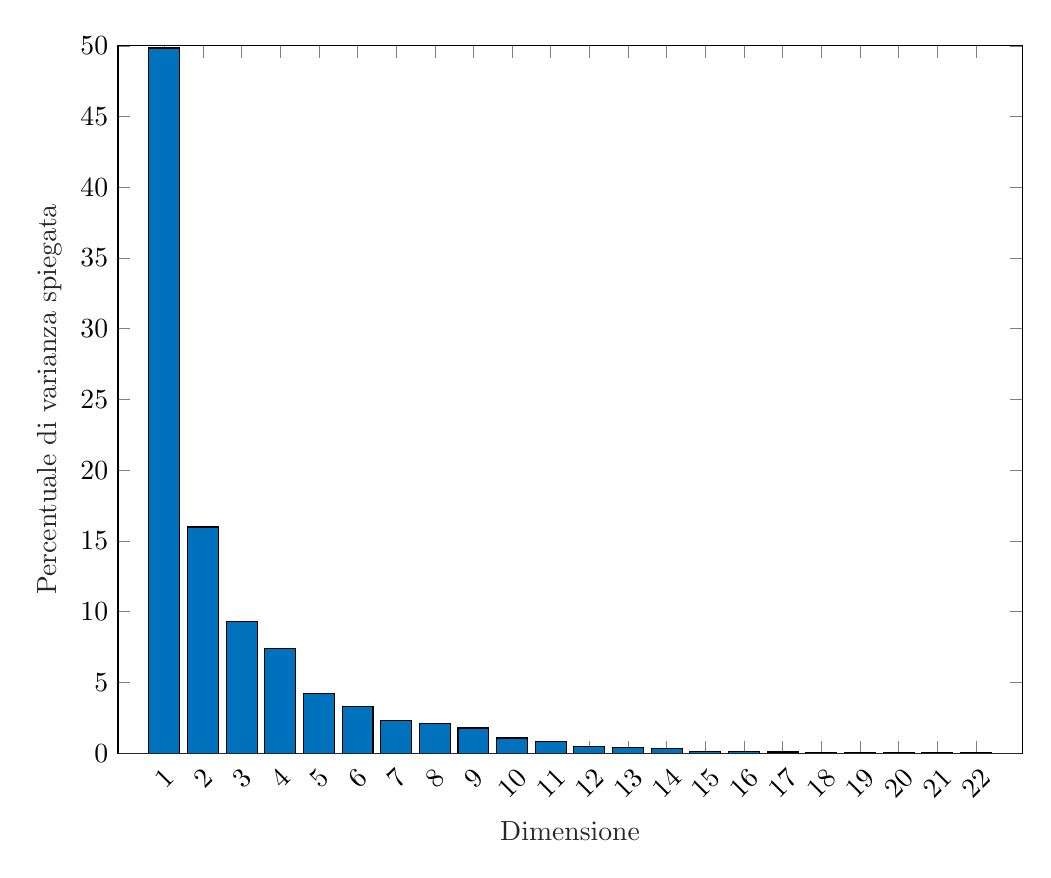
\begin{tikzpicture}

\begin{axis}[%
width=4.521in,
height=3.537in,
at={(0.758in,0.509in)},
scale only axis,
bar shift auto,
xmin=-0.2,
xmax=23.2,
xtick={ 1,  2,  3,  4,  5,  6,  7,  8,  9, 10, 11, 12, 13, 14, 15, 16, 17, 18, 19, 20, 21, 22},
xticklabel style={rotate=45},
xlabel style={font=\color{white!15!black}},
xlabel={Dimensione},
ymin=0,
ymax=50,
ylabel style={font=\color{white!15!black}},
ylabel={Percentuale di varianza spiegata},
axis background/.style={fill=white}
]
\addplot[ybar, bar width=0.8, fill=mycolor1, draw=black, area legend] table[row sep=crcr] {%
1	49.8429384140697\\
2	15.9914290649364\\
3	9.31784162651434\\
4	7.37097273589509\\
5	4.25068423484215\\
6	3.32692732033862\\
7	2.28321256413735\\
8	2.09173313220835\\
9	1.77840144968417\\
10	1.07612296977032\\
11	0.801339351846553\\
12	0.442946471601915\\
13	0.379899397362674\\
14	0.344307244279531\\
15	0.149692392485431\\
16	0.139808243561912\\
17	0.0877235268044593\\
18	0.0779778665045899\\
19	0.0635043947853086\\
20	0.0486797853759288\\
21	0.0416900664680096\\
22	0.027713995555292\\
};
\addplot[forget plot, color=white!15!black] table[row sep=crcr] {%
-0.2	0\\
23.2	0\\
};
\end{axis}
\end{tikzpicture}%